% Circumscribed Parallelepiped
% Author: Axel Pavillet
\documentclass[tikz,border=10pt]{standalone}
\usepackage{verbatim}
\usetikzlibrary{calc}
\usetikzlibrary{intersections}
\begin{document}
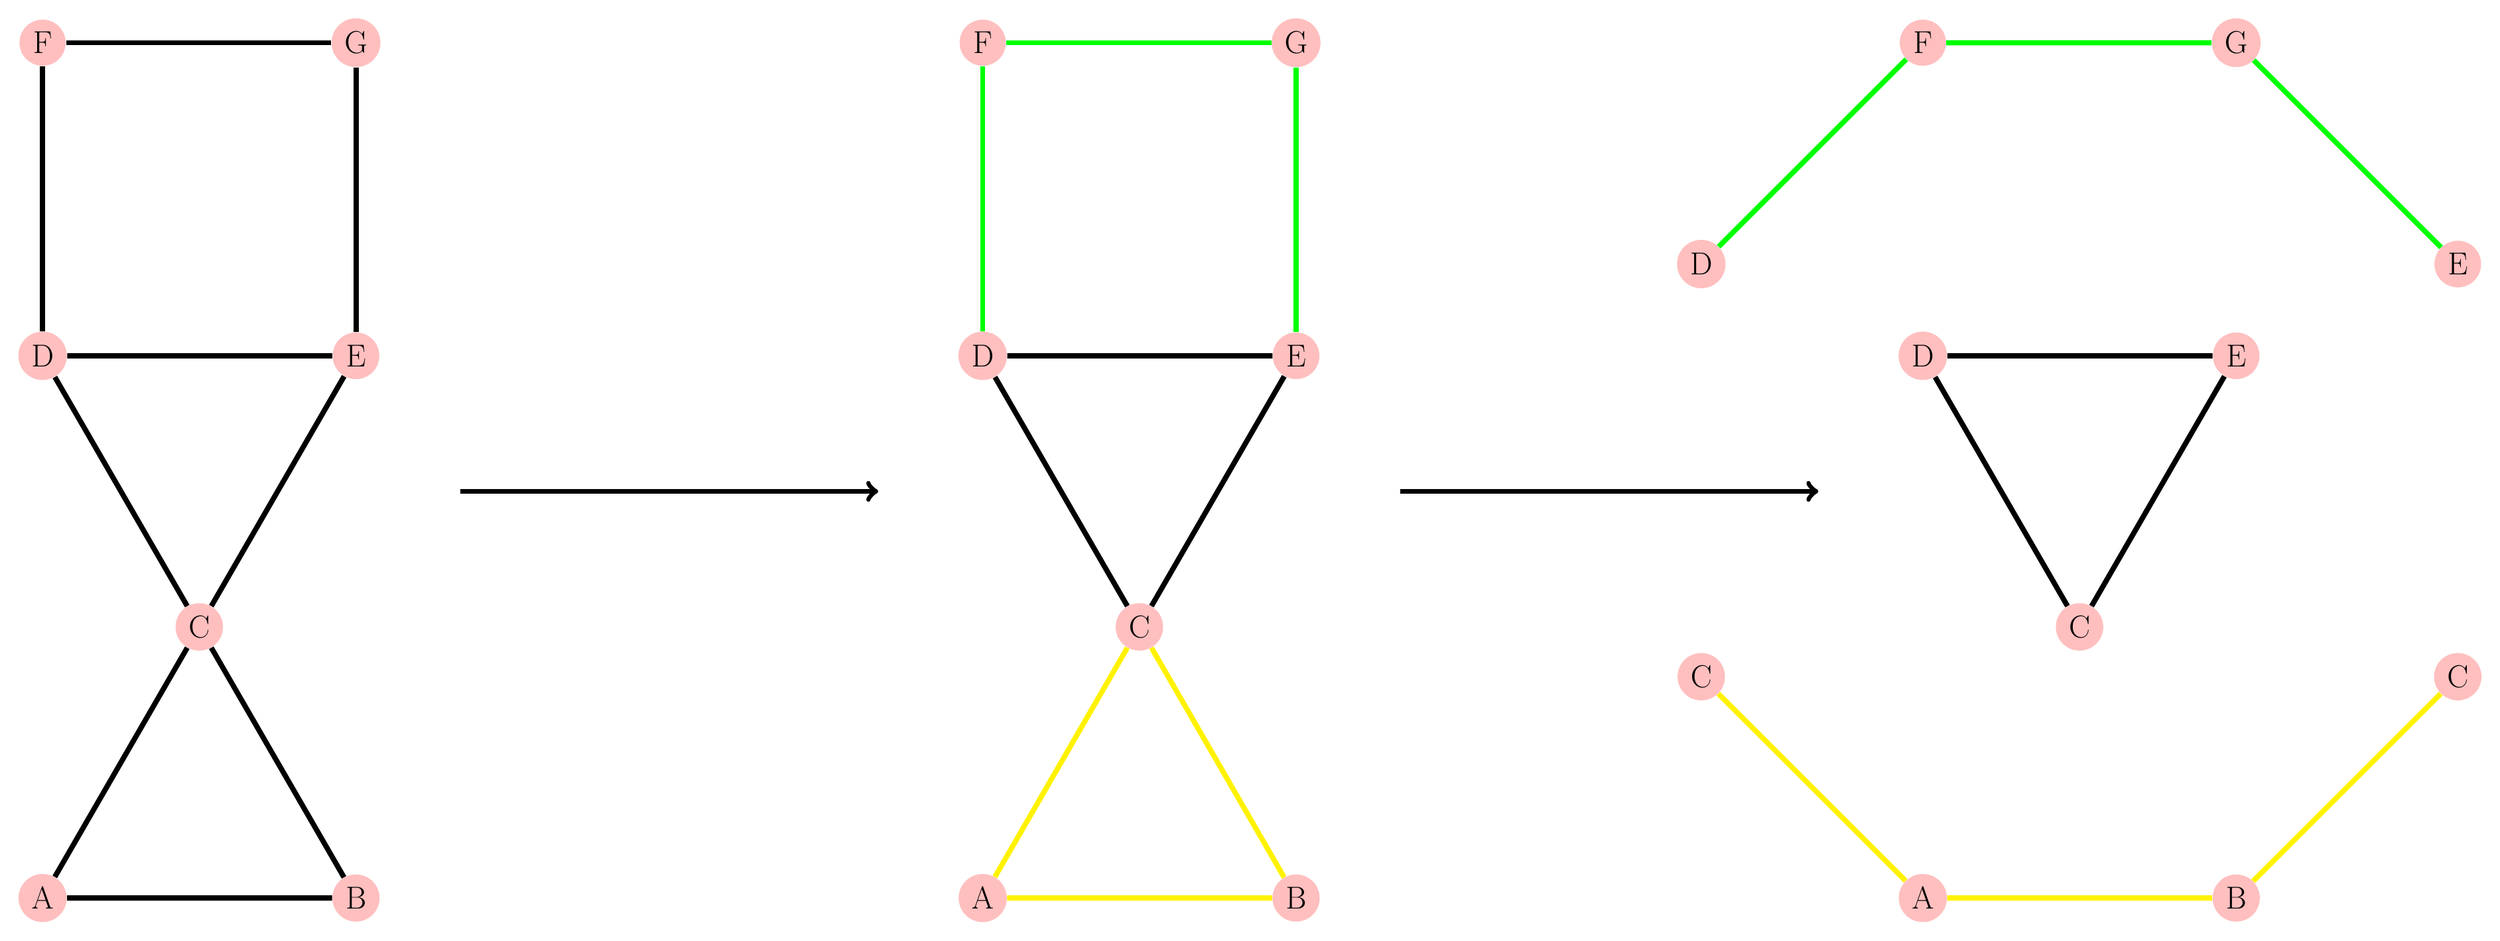
\begin{tikzpicture}[font=\LARGE]

\def\rootThree{1.732}
\def\rootTwo{1.414}
\def\ax{0} \def\bx{3} \def\cx{6} \def\dx{18} \def\ex{21} \def\fx{24} \def\gx{\dx-\cx+\fx} \def\hx{\gx+3} \def\ix{\hx+3}
\def\ay{0} \def\by{3*\rootThree} \def\cy{6*\rootThree} \def\dy{6+6*\rootThree} \def\liney{4.5*\rootThree}
\node [fill=pink,circle] (A) at (\ax,\ay) {A};
\node [fill=pink,circle] (B) at (\cx,\ay) {B};

\node [fill=pink,circle] (C) at (\bx,\by) {C};

\node [fill=pink,circle] (D) at (\ax,\cy) {D};
\node [fill=pink,circle] (E) at (\cx,\cy) {E};

\node [fill=pink,circle] (F) at (\ax,\dy) {F};
\node [fill=pink,circle] (G) at (\cx,\dy) {G};

\draw [line width=1mm] (A) -- (B) -- (C) -- (A);
\draw [line width=1mm] (C) -- (D) -- (E) -- (C);
\draw [line width=1mm] (D) -- (F) -- (G) -- (E);

\draw [->,line width=1mm] (\cx+2,\liney) -- (\dx-2,\liney);

\node [fill=pink,circle] (2_A) at (\dx,\ay) {A};
\node [fill=pink,circle] (2_B) at (\fx,\ay) {B};

\node [fill=pink,circle] (2_C) at (\ex,\by) {C};

\node [fill=pink,circle] (2_D) at (\dx,\cy) {D};
\node [fill=pink,circle] (2_E) at (\fx,\cy) {E};

\node [fill=pink,circle] (2_F) at (\dx,\dy) {F};
\node [fill=pink,circle] (2_G) at (\fx,\dy) {G};

\draw [color=yellow,line width=1mm] (2_A) -- (2_B) -- (2_C) -- (2_A);
\draw [line width=1mm] (2_C) -- (2_D) -- (2_E) -- (2_C);
\draw [color=green,line width=1mm] (2_D) -- (2_F) -- (2_G) -- (2_E);

\draw [->,line width=1mm] (\fx+2,\liney) -- (\gx-2,\liney);

\node [fill=pink,circle] (3_L_D) at (\gx-3*\rootTwo,\dy-3*\rootTwo) {D};
\node [fill=pink,circle] (3_F) at (\gx,\dy) {F};
\node [fill=pink,circle] (3_G) at (\ix,\dy) {G};
\node [fill=pink,circle] (3_R_E) at (\ix+3*\rootTwo,\dy-3*\rootTwo) {E};

\draw [color=green,line width=1mm] (3_L_D) -- (3_F) -- (3_G) -- (3_R_E);

\node [fill=pink,circle] (3_R_D) at (\gx,\cy) {D};
\node [fill=pink,circle] (3_L_E) at (\ix,\cy) {E};
\node [fill=pink,circle] (3_U_C) at (\hx,\by) {C};

\draw [line width=1mm] (3_R_D) -- (3_L_E) -- (3_U_C) -- (3_R_D);

\node [fill=pink,circle] (3_L_C) at (\gx-3*\rootTwo,\ay+3*\rootTwo) {C};
\node [fill=pink,circle] (3_A) at (\gx,\ay) {A};
\node [fill=pink,circle] (3_B) at (\ix,\ay) {B};
\node [fill=pink,circle] (3_R_C) at (\ix+3*\rootTwo,\ay+3*\rootTwo) {C};

\draw [color=yellow,line width=1mm] (3_L_C) -- (3_A) -- (3_B) -- (3_R_C);
\end{tikzpicture}
\end{document}

